\documentclass[aspectratio=169,10pt]{beamer}
\usepackage[T1]{fontenc}
\usepackage[utf8]{inputenc}
\usepackage[english]{babel}
\usepackage{amsmath,amssymb,booktabs,tikz}
\usetikzlibrary{arrows.meta,positioning}

\definecolor{Navy}{RGB}{8,20,38}
\definecolor{Teal}{RGB}{15,118,110}
\definecolor{Mint}{RGB}{45,212,191}
\definecolor{Gold}{RGB}{245,158,11}
\definecolor{Cloud}{RGB}{241,245,249}
\definecolor{Ink}{RGB}{30,41,59}
\setbeamercolor{normal text}{fg=Ink,bg=white}
\setbeamercolor{structure}{fg=Teal}
\setbeamercolor{frametitle}{fg=white,bg=Navy}
\setbeamercolor{block title}{fg=white,bg=Teal}
\setbeamercolor{block body}{fg=Ink,bg=Cloud}
\setbeamercolor{alerted text}{fg=Gold}
\setbeamertemplate{navigation symbols}{}
\setbeamertemplate{itemize item}{\color{Mint}$\blacktriangleright$}
\setbeamertemplate{footline}{\leavevmode\hbox{%
  \begin{beamercolorbox}[wd=.83\paperwidth,ht=2.7ex,dp=1.1ex,leftskip=1em]{author in head/foot}\color{white!80!Navy}Quispe \& Xu (2026) · short deck\end{beamercolorbox}%
  \begin{beamercolorbox}[wd=.17\paperwidth,ht=2.7ex,dp=1.1ex,center]{date in head/foot}\insertframenumber/\inserttotalframenumber\end{beamercolorbox}}}

\title{Agentic Delegation and the Language Frontier}
\subtitle{A model and evidence from Claude Code on GitHub}
\author{John Barraza}
\institute{AI Economic Modelling · Repository 03}
\date{September 2026}

\begin{document}

\begin{frame}[plain]
  \begin{tikzpicture}[remember picture,overlay]
    \fill[Navy] (current page.south west) rectangle (current page.north east);
    \fill[Teal] ([xshift=.62\paperwidth]current page.south west) rectangle (current page.north east);
    \fill[Gold,opacity=.75] ([xshift=.70\paperwidth,yshift=.19\paperheight]current page.south west) rectangle ([xshift=.82\paperwidth,yshift=.50\paperheight]current page.south west);
  \end{tikzpicture}
  \color{white}\vspace{1.3em}
  {\Huge\bfseries Agentic Delegation}\par\vspace{.35em}
  {\Large and the Language Frontier}\par\vspace{1.3em}
  {\large Quispe \& Xu (2026), arXiv:2605.25438v2}\par
  \vfill
  {\small John Barraza · \url{https://github.com/johnbarraza/ai-03-quispe}}
\end{frame}

\begin{frame}{Question and correction}
  \begin{block}{Question}
  Does agentic AI expand the set of programming languages in which a developer can ship code, rather than only accelerating familiar work?
  \end{block}
  \vspace{.5em}
  \textbf{Citation audit.} The current paper has two authors, Alexander Quispe and Kevin Xu, and a new title. It is a preliminary, unrefereed \alert{arXiv preprint}, not an NBER paper.
  \vspace{.7em}
  \textbf{Claim boundary.} This is a \alert{production frontier}, not proof that the developer learns an unfamiliar language.
\end{frame}

\begin{frame}{Three capabilities, one threshold mechanism}
  \begin{columns}[T,onlytextwidth]
  \begin{column}{.31\textwidth}\begin{block}{Solo $S$}Human executes with language-specific skill $s$.\end{block}\end{column}
  \begin{column}{.31\textwidth}\begin{block}{Augment $C$}Suggestions help in proportion to the foothold $s$.\end{block}\end{column}
  \begin{column}{.31\textwidth}\begin{block}{Delegate $D$}Agent executes; human specifies and verifies using general ability $a$.\end{block}\end{column}
  \end{columns}
  \vspace{.8em}
  \[
  M^1=\{S,C\}\subset M^2=\{S,C,D\},\qquad
  Z^g=\mathbf 1\!\left\{\max_{m\in M^g}V^m\ge0\right\}.
  \]
  \centering\small The core model has discrete mode choice and entry---\textbf{no continuous effort choice}.
\end{frame}

\begin{frame}{Main result: an activation band}
  For an unfamiliar language, augmentation needs a foothold:
  \[
  \gamma s-r_C\le0\quad\Longrightarrow\quad T^1=T^S.
  \]
  If delegation lowers the threshold, $B=T^S-T^D>0$, then
  \[
  \boxed{Z^2-Z^1=\mathbf 1\{T^D\le\omega<T^1\}}.
  \]
  \begin{center}
  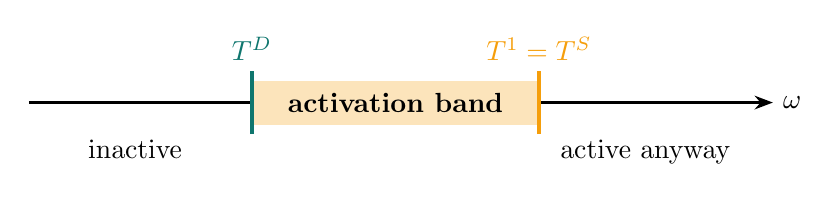
\begin{tikzpicture}[x=1.35cm,y=1cm]
    \draw[-{Stealth},thick] (0,0)--(7,0) node[right]{$\omega$};
    \fill[Gold!28] (2.1,-.28) rectangle (4.8,.28);
    \draw[Teal,very thick] (2.1,-.4)--(2.1,.4) node[above]{$T^D$};
    \draw[Gold,very thick] (4.8,-.4)--(4.8,.4) node[above]{$T^1=T^S$};
    \node at (3.45,0) {\bfseries activation band};
    \node[below] at (1,-.35) {inactive}; \node[below] at (5.8,-.35) {active anyway};
  \end{tikzpicture}
  \end{center}
\end{frame}

\begin{frame}{Data and design}
  \begin{columns}[T,onlytextwidth]
  \begin{column}{.48\textwidth}
    \begin{block}{Estimation panel}
    \textbf{5,346} developers: 2,813 treated and 2,533 not-yet-treated controls; 28 months and 149,688 rows.
    \end{block}
    \textbf{Measurement:} 3.2m commits, 133k developer--repository pairs, and \textbf{57m changed files} classified with GitHub Linguist.
  \end{column}
  \begin{column}{.48\textwidth}
    Adoption is first detectable Claude co-authorship. Estimation uses doubly robust staggered DiD, one-month anticipation, and developer-clustered bootstrap SEs.
    \vspace{.7em}
    \begin{alertblock}{Identification}
    Voluntary adoption may coincide with a new unfamiliar-language project. Estimates are associations, not definitive causal effects.
    \end{alertblock}
  \end{column}
  \end{columns}
\end{frame}

\begin{frame}{What happens at adoption?}
  \centering\small
  \begin{tabular}{lrrl}
  \toprule
  Outcome & ATT at $e=0$ & SE & Benchmark \\
  \midrule
  Active languages & \textbf{2.528} & .063 & pre-mean .90 \\
  Newly used languages & \textbf{1.193} & .051 & pre-flow .31 \\
  Language entropy & \textbf{.382} & .009 & pre-mean .15 \\
  Cumulative languages & \textbf{1.604} & .054 & 2.072 by $e=2$ \\
  Monthly commits & 35.080 & 2.085 & diagnostic \\
  \bottomrule
  \end{tabular}
  \vspace{1em}
  \begin{block}{Stock--flow signature}
  New-language entry spikes and reverts; cumulative language breadth continues growing. Specialists add far more new languages than generalists within activity groups.
  \end{block}
\end{frame}

\begin{frame}{Economic conclusion}
  \Large
  Agentic delegation can turn \alert{general specification-and-verification ability} into production across domains where specialized execution skill is scarce.
  \vspace{1em}

  \normalsize
  Robustness checks and specialist heterogeneity support the mechanism. They do not eliminate selection into adoption or prove skill acquisition.
  \vfill
  \small Full derivations, SymPy audit, and extended deck: \url{https://github.com/johnbarraza/ai-03-quispe}
\end{frame}

\end{document}

